%
% Time domain
%
In order to define and to work with time it is necessary to study and understand the underlying domain. Moreover, the definition of a temporal domain is the basis for almost any temporal system. In the following subsection \ref{subsec:basic-concepts} we will introduce several concepts that are widely used in the community of temporal databases. Most of the concepts explained here have been introduced in the \emph{'Consensus Glossary of Temporal Database Concepts'}~\cite{Dyreson1994}.



\subsection{Basic concepts and properties}
\label{subsec:basic-concepts}

Time is usually represented as a set with an imposed partial order. There are two main models of time: \textbf{linear} and \textbf{cyclic}. In the linear model, time advances from the past to the future in a totally ordered fashion (a relationship of total order is imposed to the set). A cyclic model of time is used for recurrent processes. The majority of the proposals work with a linear model of time.

\begin{svgraybox}
The basic elements in a temporal domain are the following:\\
%\begin{itemize}
%\item
\textbf{Instant}:  Is a time point over an underlying temporal domain.\\
%\item
\textbf{Time interval}: Is the time between two instants.\\
%\item
\textbf{Event}: Is an instantaneous fact. Something that happens at an instant.\\
%\item
\textbf{Chronon}: Is a non-decomposable time interval of fixed duration. It is possible for a temporal model to leave the chronon duration unspecified. The duration will be specified later in the implementation of the model.
%\end{itemize}
\end{svgraybox}

\begin{definition}\textbf{(set of chronons)}
\label{def:set-chronon}
The \textbf{\emph{set of all the chronons}} in a system is denoted by $\C$. A chronon $c$ is therefore defined as:
\begin{equation}
\left \lbrace c \mid c \in \C \right \rbrace
\end{equation}
\end{definition}

Any temporal model may represent the time as points as well as intervals. The equivalence between a interval-based and point-based temporal data models is demonstrated in \cite{Böhlen_point-versus}.

Attending to the density in the set $\C$ of the chronons, a model can be classified into the following three types:

\begin{itemize}
\item
\textbf{Discrete model} ($\C \subset \Nat$):  The discrete model of time is isomorphic in relation to the natural numbers. According to this model, each natural number corresponds to a \emph{chronon}.
\item
\textbf{Dense model} ($\C \subset \Q$ or $\C \subset \R$): This model is isomorphic in relation to the rational or the real numbers. It represents one instant of time in the gap between another two instants. 
\item
\textbf{Continuous model} ($\C \subset \R$): This is an extension of the dense model with no gaps. It is isomorphic in relation to the real numbers. 
\end{itemize}




Restrictions on time range may be performed on the base of the following two concepts:
\begin{itemize}
\item
\textbf{Time boundedness}: Time can be bounded orthogonally in the past and in the future.
\item
\textbf{Time distance}: As a metric, time has a distance function which presents four properties:
\begin{enumerate}
\item
Distance is non-negative.
\item
The distance between two different elements is not equal to zero.
\item
The distance from $\alpha$ to $\beta$ is the same as that between $\beta$ and $\alpha$.
\item
Triangle inequality: The distance from $\alpha$ to $\gamma$ is equal or greater than the distance from $\alpha$ to $\beta$ plus the distance from $\beta$ to $\gamma$.
\end{enumerate}
\end{itemize}

On the other hand, time may be \textbf{relative} or \textbf{absolute} (in other words, \textbf{anchored} or \textbf{unanchored}). Sometimes, what one considers \emph{absolute time} is not as definite as one would hope since our concept of absolute time is based on another time reference (for example, January 1st of year one). Relative time has a direction, differently from distance. It is also possible to use negative references so as to represent relative time (e.g. -3 days = three days ago).


%%% granularity
\subsection{\label{subsec:granularity}Granularity}
Next to the inherent difficulties of time, an issue is \textbf{temporal granularity}. A temporal granularity is a partitioning of the time line used by a system, usually dependent on the application. For example, the age of an adult human being is usually expressed in years: one will use sentences like \emph{`Laura is 21 years old'} instead of \emph{`Laura is 21 years, 3 months and 4 days old'}. In this example any time period shorter than a year needs no representation and thus the used granularity allows no specification for time periods shorter than a year.
The formal definition for granularity is given in ~\cite{Lin97}:


\begin{definition}
\label{def:granularity}\textbf{(granularity)}
A \textbf{\emph{granularity}} $\alpha$ is an ordered set of non-overlapping and continuous time elements called granules. \\
\end{definition}

\begin{definition}
\label{def:granule}\textbf{(granule)}
A \textbf{\emph{granule}} is the basic time unit represented by a granularity. E.g. in the hours granularity, an hour is a granule.
As granularity $\alpha$ it is an ordered set, each \emph{granule} may be indexed by an integer number:\\
\begin{equation}
\alpha = \left \lbrace \ldots, 0_\alpha, 1_\alpha, \ldots \right \rbrace
\end{equation}
\end{definition}

In a system, the smallest granularity is the \emph{chronons} granularity, denoted with the index $\bot$. It is possible to define a function $f$ that maps from  a given granule $i_\alpha$ (in the given granularity $\alpha$) to the set of the corresponding chronons. 

\begin{definition}
\label{def:mapping-function}
\textbf{(mapping function)}
The \textbf{\emph{mapping function}} $f$ in a given granule $i_\alpha$ is denoted by:\\
%\begin{align}
$f:i_\alpha \rightarrow \C$\\
$f(i_\alpha) = \lbrace c_\bot \mid c_\bot$ is in $i_\alpha \rbrace \wedge c_\bot \in \C$\\
%\end{align}
\end{definition}


If $\alpha$ is a granularity, then the following properties must hold:\\
\begin{itemize}
\item
$\alpha$ is an ordered set: if $c_\bot \in f(i_\alpha)$ and $c^{'}_\bot \in f(j_\alpha)$ and $c_\bot < c^{'}_\bot$ implies that $i_\alpha < j_\alpha$.
\begin{figure}
\centering
%%Created by jPicEdt 1.4.1_03: mixed JPIC-XML/LaTeX format
%%Mon Jan 30 18:36:37 CET 2012
%%Begin JPIC-XML
%<?xml version="1.0" standalone="yes"?>
%<jpic x-min="-5" x-max="50" y-min="-2" y-max="22" auto-bounding="true">
%<multicurve fill-style= "none"
%	 points= "(0,0);(0,0);(50,0);(50,0)"
%	 />
%<multicurve fill-style= "none"
%	 points= "(0,20);(0,20);(50,20);(50,20)"
%	 />
%<multicurve fill-style= "none"
%	 points= "(2,0);(2,0);(10,20);(10,20)"
%	 />
%<multicurve fill-style= "none"
%	 points= "(10,20);(10,20);(16,0);(16,0)"
%	 />
%<multicurve fill-style= "none"
%	 points= "(24,0);(24,0);(32,20);(32,20)"
%	 />
%<multicurve fill-style= "none"
%	 points= "(32,20);(32,20);(38,0);(38,0)"
%	 />
%<text text-vert-align= "center-v"
%	 anchor-point= "(10,22)"
%	 fill-style= "none"
%	 text-frame= "noframe"
%	 text-hor-align= "center-h"
%	 >
%$i_G$
%</text>
%<text text-vert-align= "center-v"
%	 anchor-point= "(32,22)"
%	 fill-style= "none"
%	 text-frame= "noframe"
%	 text-hor-align= "center-h"
%	 >
%$j_G$
%</text>
%<text text-vert-align= "center-v"
%	 anchor-point= "(8,-2)"
%	 fill-style= "none"
%	 text-frame= "noframe"
%	 text-hor-align= "center-h"
%	 >
%$c_\bot$
%</text>
%<text text-vert-align= "center-v"
%	 anchor-point= "(34,-2)"
%	 fill-style= "none"
%	 text-frame= "noframe"
%	 text-hor-align= "center-h"
%	 >
%$c^{'}_\bot$
%</text>
%<text text-vert-align= "center-v"
%	 anchor-point= "(0,10)"
%	 fill-style= "none"
%	 text-frame= "noframe"
%	 text-hor-align= "center-h"
%	 >
%$f(i_G)$
%</text>
%<text text-vert-align= "center-v"
%	 anchor-point= "(42,10)"
%	 fill-style= "none"
%	 text-frame= "noframe"
%	 text-hor-align= "center-h"
%	 >
%$f(j_G)$
%</text>
%<text text-vert-align= "center-v"
%	 anchor-point= "(-5,0)"
%	 fill-style= "none"
%	 text-frame= "noframe"
%	 text-hor-align= "center-h"
%	 >
%$\C$
%</text>
%<text text-vert-align= "center-v"
%	 anchor-point= "(-5,20)"
%	 fill-style= "none"
%	 text-frame= "noframe"
%	 text-hor-align= "center-h"
%	 >
%$G$
%</text>
%</jpic>
%%End JPIC-XML
%LaTeX-picture environment using emulated lines and arcs
%You can rescale the whole picture (to 80% for instance) by using the command \def\JPicScale{0.8}
\ifx\JPicScale\undefined\def\JPicScale{1}\fi
\unitlength \JPicScale mm
\begin{picture}(50,22)(0,0)
\linethickness{0.3mm}
\put(0,0){\line(1,0){50}}
\linethickness{0.3mm}
\put(0,20){\line(1,0){50}}
\linethickness{0.3mm}
\multiput(2,0)(0.12,0.3){67}{\line(0,1){0.3}}
\linethickness{0.3mm}
\multiput(10,20)(0.12,-0.4){50}{\line(0,-1){0.4}}
\linethickness{0.3mm}
\multiput(24,0)(0.12,0.3){67}{\line(0,1){0.3}}
\linethickness{0.3mm}
\multiput(32,20)(0.12,-0.4){50}{\line(0,-1){0.4}}
\put(10,22){\makebox(0,0)[cc]{$i_G$}}

\put(32,22){\makebox(0,0)[cc]{$j_G$}}

\put(8,-2){\makebox(0,0)[cc]{$c_\bot$}}

\put(34,-2){\makebox(0,0)[cc]{$c^{'}_\bot$}}

\put(0,10){\makebox(0,0)[cc]{$f(i_G)$}}

\put(42,10){\makebox(0,0)[cc]{$f(j_G)$}}

\put(-5,0){\makebox(0,0)[cc]{$\C$}}

\put(-5,20){\makebox(0,0)[cc]{$G$}}

\end{picture}

\caption{$\alpha$ is an ordered set}
\label{fig:granularity-prop1}
\end{figure}
\item
$\alpha$ is a set of continuous granules. Consider the chronons $c_\bot < c^{'}_\bot < c^{''}_\bot$. Then $c_\bot \in f(i_\alpha)$,$c^{''}_\bot \in f(i_\alpha)$ implies that $c^{'}_\bot \in f(i_\alpha)$.
\begin{figure}
\centering
%%Created by jPicEdt 1.4.1_03: mixed JPIC-XML/LaTeX format
%%Tue Jan 17 10:05:05 CET 2012
%%Begin JPIC-XML
%<?xml version="1.0" standalone="yes"?>
%<jpic x-min="-4" x-max="50" y-min="-2" y-max="20" auto-bounding="true">
%<multicurve fill-style= "none"
%	 points= "(0,0);(0,0);(50,0);(50,0)"
%	 />
%<multicurve fill-style= "none"
%	 points= "(0,20);(0,20);(50,20);(50,20)"
%	 />
%<text text-vert-align= "center-v"
%	 anchor-point= "(-4,20)"
%	 fill-style= "none"
%	 text-frame= "noframe"
%	 text-hor-align= "center-h"
%	 >
%$\alpha$
%</text>
%<text text-vert-align= "center-v"
%	 anchor-point= "(-4,0)"
%	 fill-style= "none"
%	 text-frame= "noframe"
%	 text-hor-align= "center-h"
%	 >
%$\C$
%</text>
%<multicurve fill-style= "none"
%	 points= "(14,0);(14,0);(22,20);(22,20)"
%	 />
%<multicurve fill-style= "none"
%	 points= "(22,20);(22,20);(28,0);(28,0)"
%	 />
%<text text-vert-align= "center-v"
%	 anchor-point= "(10,10)"
%	 fill-style= "none"
%	 text-frame= "noframe"
%	 text-hor-align= "center-h"
%	 >
%$f(i_\alpha)$
%</text>
%<text text-vert-align= "center-v"
%	 anchor-point= "(16,-2)"
%	 fill-style= "none"
%	 text-frame= "noframe"
%	 text-hor-align= "center-h"
%	 >
%$c_\bot$
%</text>
%<text text-vert-align= "center-v"
%	 anchor-point= "(20,-2)"
%	 fill-style= "none"
%	 text-frame= "noframe"
%	 text-hor-align= "center-h"
%	 >
%$c^{'}_\bot$
%</text>
%<text text-vert-align= "center-v"
%	 anchor-point= "(26,-2)"
%	 fill-style= "none"
%	 text-frame= "noframe"
%	 text-hor-align= "center-h"
%	 >
%$c^{''}_\bot$
%</text>
%</jpic>
%%End JPIC-XML
%LaTeX-picture environment using emulated lines and arcs
%You can rescale the whole picture (to 80% for instance) by using the command \def\JPicScale{0.8}
\ifx\JPicScale\undefined\def\JPicScale{1}\fi
\unitlength \JPicScale mm
\begin{picture}(50,20)(0,0)
\linethickness{0.3mm}
\put(0,0){\line(1,0){50}}
\linethickness{0.3mm}
\put(0,20){\line(1,0){50}}
\put(-4,20){\makebox(0,0)[cc]{$\alpha$}}

\put(-4,0){\makebox(0,0)[cc]{$\C$}}

\linethickness{0.3mm}
\multiput(14,0)(0.12,0.3){67}{\line(0,1){0.3}}
\linethickness{0.3mm}
\multiput(22,20)(0.12,-0.4){50}{\line(0,-1){0.4}}
\put(10,10){\makebox(0,0)[cc]{$f(i_\alpha)$}}

\put(16,-2){\makebox(0,0)[cc]{$c_\bot$}}

\put(20,-2){\makebox(0,0)[cc]{$c^{'}_\bot$}}

\put(26,-2){\makebox(0,0)[cc]{$c^{''}_\bot$}}

\end{picture}

\caption{$\alpha$ is a set of continuous granules}
\label{fig:granularity-prop2}
\end{figure}
\item
The granules in $\alpha$ do not overlap: If $i_\alpha \neq j_\alpha$ then $f(i_\alpha) \cap f(j_\alpha) = \emptyset$.
\begin{figure}
\centering
%%Created by jPicEdt 1.4.1_03: mixed JPIC-XML/LaTeX format
%%Tue Jan 17 10:05:40 CET 2012
%%Begin JPIC-XML
%<?xml version="1.0" standalone="yes"?>
%<jpic x-min="-4" x-max="50" y-min="0" y-max="22" auto-bounding="true">
%<multicurve fill-style= "none"
%	 points= "(0,0);(0,0);(50,0);(50,0)"
%	 />
%<multicurve fill-style= "none"
%	 points= "(0,20);(0,20);(50,20);(50,20)"
%	 />
%<text text-vert-align= "center-v"
%	 anchor-point= "(-4,20)"
%	 fill-style= "none"
%	 text-frame= "noframe"
%	 text-hor-align= "center-h"
%	 >
%$\alpha$
%</text>
%<text text-vert-align= "center-v"
%	 anchor-point= "(-4,0)"
%	 fill-style= "none"
%	 text-frame= "noframe"
%	 text-hor-align= "center-h"
%	 >
%$\C$
%</text>
%<multicurve fill-style= "none"
%	 points= "(4,0);(4,0);(12,20);(12,20)"
%	 />
%<multicurve fill-style= "none"
%	 points= "(12,20);(12,20);(18,0);(18,0)"
%	 />
%<multicurve fill-style= "none"
%	 points= "(28,0);(28,0);(36,20);(36,20)"
%	 />
%<multicurve fill-style= "none"
%	 points= "(36,20);(36,20);(42,0);(42,0)"
%	 />
%<text text-vert-align= "center-v"
%	 anchor-point= "(2,10)"
%	 fill-style= "none"
%	 text-frame= "noframe"
%	 text-hor-align= "center-h"
%	 >
%$f(i_\alpha)$
%</text>
%<text text-vert-align= "center-v"
%	 anchor-point= "(46,10)"
%	 fill-style= "none"
%	 text-frame= "noframe"
%	 text-hor-align= "center-h"
%	 >
%$f(j_\alpha)$
%</text>
%<text text-vert-align= "center-v"
%	 anchor-point= "(12,22)"
%	 fill-style= "none"
%	 text-frame= "noframe"
%	 text-hor-align= "center-h"
%	 >
%$i_\alpha$
%</text>
%<text text-vert-align= "center-v"
%	 anchor-point= "(36,22)"
%	 fill-style= "none"
%	 text-frame= "noframe"
%	 text-hor-align= "center-h"
%	 >
%$j_\alpha$
%</text>
%</jpic>
%%End JPIC-XML
%LaTeX-picture environment using emulated lines and arcs
%You can rescale the whole picture (to 80% for instance) by using the command \def\JPicScale{0.8}
\ifx\JPicScale\undefined\def\JPicScale{1}\fi
\unitlength \JPicScale mm
\begin{picture}(50,22)(0,0)
\linethickness{0.3mm}
\put(0,0){\line(1,0){50}}
\linethickness{0.3mm}
\put(0,20){\line(1,0){50}}
\put(-4,20){\makebox(0,0)[cc]{$\alpha$}}

\put(-4,0){\makebox(0,0)[cc]{$\C$}}

\linethickness{0.3mm}
\multiput(4,0)(0.12,0.3){67}{\line(0,1){0.3}}
\linethickness{0.3mm}
\multiput(12,20)(0.12,-0.4){50}{\line(0,-1){0.4}}
\linethickness{0.3mm}
\multiput(28,0)(0.12,0.3){67}{\line(0,1){0.3}}
\linethickness{0.3mm}
\multiput(36,20)(0.12,-0.4){50}{\line(0,-1){0.4}}
\put(2,10){\makebox(0,0)[cc]{$f(i_\alpha)$}}

\put(46,10){\makebox(0,0)[cc]{$f(j_\alpha)$}}

\put(12,22){\makebox(0,0)[cc]{$i_\alpha$}}

\put(36,22){\makebox(0,0)[cc]{$j_\alpha$}}

\end{picture}

\caption{The granules in $\alpha$ do not overlap}
\label{fig:granularity-prop3}
\end{figure}
\end{itemize}

The mapping function $f$ allows the comparison among granularities:

\begin{definition}
\label{def:finner-than}\textbf{(finner than)}
A granularity $\alpha$ is \emph{``finner than''} granularity $\beta$ when the set of corresponding chronons for a given granule $i_\alpha$ is smaller than the set of the corresponding chronons for a given granule $j_\beta$.
\begin{equation}
\label{eq:finner-than}
\mid f \left( i_\alpha \right) \mid < \mid  f \left( j_\beta \right) \mid
\end{equation} 
\end{definition}

\begin{definition}
\label{def:coarser-than}\textbf{(coarser than)}
A granularity $\alpha$ is \emph{``coarser than''} granularity $\beta$ when the set of corresponding chronons for a given granule $i_\alpha$ is greater than the set of the corresponding chronons for a given granule $j_\beta$.
\begin{equation}
\label{eq:coarser-than}
\mid f \left( i_\alpha \right) \mid > \mid  f \left( j_\beta \right) \mid
\end{equation} 
\end{definition}




A function,\emph{Cast} may be specified to map between two granularities $\alpha$ and $\beta$. The specification for that function is:
\begin{equation}
\label{eq:cast-function}
\mbox{Cast} \left( i_\alpha,\alpha,\beta \right) = j_\beta
\end{equation}
This function associates a granule $i_\alpha$ in the granularity $\alpha$ to a corresponding granule $j_\beta$ in the corresponding granularity $\beta$. An \emph{upwards mapping} is the mapping from a granularity $\alpha$ to a coarser granularity $\beta$, whereas a downwards mapping is the mapping from a granularity $\gamma$ to a finner granularity $\delta$. Figure \ref{fig:granularity-graph-example} shows a granularity graph example with the Gregorian Calendar and the academic days as possible granularities.

\begin{figure}
\centering
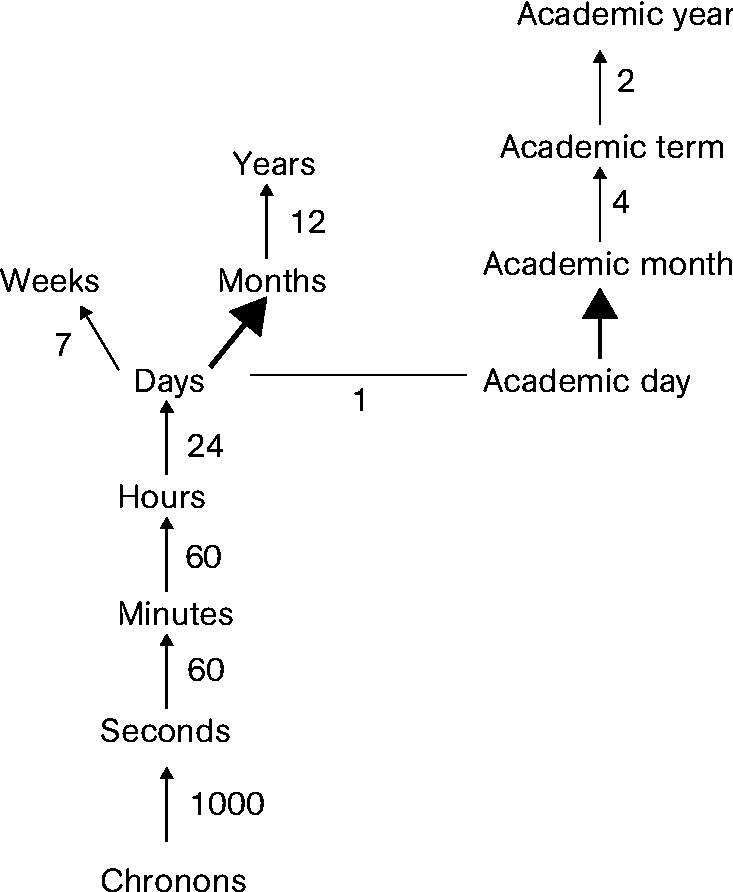
\includegraphics[scale=0.5]{graphs/granularityGraph.pdf}
\caption{A granularity graph example}
\label{fig:granularity-graph-example}
\end{figure}

The mapping between two granularities may be classified into the following types and are explained within the figure \ref{fig:granularity-graph-example}:
\begin{itemize}
\item
Regular mapping: When the mapping function between two granularities is calculated by means of multiplications or divisions and maybe some anchor adjustment. E.g. the mapping between hours and minutes. This mapping is represented in the figure with a normal arrow.
\item
Irregular mapping: When the mapping function can not be calculated by means of multiplications or divisions. E.g. the mapping between months and days. (This mapping is represented in the figure with a bold arrow.
\item
Congruent mapping: Two granularities that have the same granules but with different anchos. E.g. the mapping between the Gregorian Calendar and academic days. This mapping is represented in the figure with a straight line without arrow.
\end{itemize}

The transition between granularities~\cite{Lin97} is also considered as a source of imprecision. In a sentence like \emph{`The Alhambra is 612 years old'}, the temporal notion is very precise if time periods shorter than a year are irrelevant in the used granularity. However, if one is concerned with the exact day on which the last stone of the building is laid, a transition to a finer granularity, allowing the specification of time periods shorter than a year, is needed. Therefore, some proposals consider granularity as the base of the temporal model~\cite{Cru97}.



\subsection{\label{subsec:timedomain-calendar}Time domain: Calendars}
%maybe introduce previously the concept of time units, linear hierarchy and time point.
A Calendar is a organization of different granularities (e.g. day, month, year) in a hierarchy. 
In order to define a calendar, some previous concepts should be introduced~\cite{Kraus1997}:

\begin{definition}
\label{def:granularity-hierarchy}
\textbf{(Linear hierarchy of granularities)} A linear hierarchy of granularities is a finite collection of granularities with a linear order $\sqsubset$ among these granularities. The coarser granularity is called the top of the hierarchy and it must be an infinite set while all the others granularities must be finite sets.
\end{definition}

The hierarchy of days $\sqsubset$ months $\sqsubset$ years defines a linear hierarchy.

\begin{definition}
\label{def:linear-calendar}
\textbf{(Linear Calendar)} A linear calendar consist of a linear hierarchy $H$ of granularities and a validity predicate which specifies if a granule is valid in  the calendar.
\end{definition}

The linear hierarchy days $\sqsubset$ months $\sqsubset$ years represents a linear calendar. It is necessary to define the validity predicates because 17 January 2012 is a valid element of the calendar whereas 30 February 2012 is not.
 
\subsubsection{\label{subsubsubsec:julian-day-number}An example of temporal domain: Julian Day Number}
% proposal for the underlying Julian Day Number domain.

The Julian Day number \emph{JDN} \cite{Dir96} is a counter. Its value is incremented in one unit every day from 1 January 4713 B.C. at 12:00 noon. The particularity of starting at noon was useful for astronomers: the observations they took one night belonged to the same Julian Day.\\
Note that the Julian Day represents whole days. There is an extension that allows to represent any precision needed (it is called Julian Date). By default, a Julian Day is expressed in Universal Time. (U.T, also known as Solar Time). However, there are representations in Terrestrial Time (T.T), Epheris Time (J.E.D. or J.D.E.). Any time scale different from Universal Time must be explicited after the Julian Day number. There are several conversion formulas~\cite{Usn}\cite{Wik}\cite{Lea} between a date in Gregorian calendar  format and a date in  JDN format. The inverse conversion formula is proposed in~\cite{Fliegel:1968:LEM:364096.364097}\\

There are many alternatives to optimize the representation of Julian Day numbers because of its extremely far origin (4713 B.C. year). Table \ref{table:juliandayrepresentations} shows several time domains that can be calculated from the Julian Date, some of them are proposed just for optimization purposes.


\begin{table}
\caption{Julian Day representations}
\label{table:juliandayrepresentations}

\begin{tabular}{p{2cm}p{4cm}p{4cm}p{2cm}}
%header ------------------------------------------------------
\hline\noalign{\smallskip}
Name & From & Formula & Current Value  \\ 
\noalign{\smallskip}\svhline\noalign{\smallskip}
%header ------------------------------------------------------
Julian Date (JD)$^a$ & 12:00 noon Monday 1 January 4713 B.C & & 2455278. 85488  \\ 
Julian Day Number (JDN)$^b$ & 12:00 noon  Monday 1 January 4713 B.C. & JND = floor(JD) & 2455278 \\ 
Reduced Julian Day (RJD)$^c$ & 12:00 noon Tuesday 16 November 1858 A.C. & RJD = JD - 2400000 & 55278.85488  \\ 
Modified Julian Day (MJD)$^d$ & 00:00 Wednesday 17 November 1858 A.C. & MJD = JD - 2400000,5 & 55278.35488 \\ 
Truncated Julian Day (TJD)$^e$ & 00:00 Friday 24 May 1968 A.C. & TJD = JD - 2440000,5 & 15278.35488  \\ 
Truncated Julian Day (TJD)$^f$ & 00:00 Thursday 10 November 1995 A.C. & TJD = (JD- 0,5) mod 10000 & 5278. 35488   \\ 
Dublin Julian Day (DJD))$^g$ & 12:00 noon Sunday 31 December 1899 A.C. & DJD = JD - 2415020 & 40258. 85488 \\ 
Chronological Julian Day (CJD)$^h$  & 00:00 Monday 1 January 4713 B.C. & CJD = JD + 0,5 + timezone adjust. & 2455279. 3548843 (UT)  \\ 
Lilian Day Number$^i$ & Friday 15 October 1582 & floor(JD-2299160,5) & 156118 \\ 
ANSI Date$^j$  & Monday 1 January 1601 & floor(JD-2305812,5) & 149466  \\ 
Rata die$^k$  & Monday 1 January 1 A.C & floor(JD - 1721424.5) & 733854 \\ 
Unix time$^l$  & Thursday 1 January 1970 A.C. & (JD – 2440587.5) × 86400 & 1269333062 \\ 
\noalign{\smallskip}\hline\noalign{\smallskip}
\end{tabular}
$^a$ This is an extension of the Julian Day that allows time representation. \\
$^b$  Each day changes at noon. \\
$^c$  Used by astronomers. \\
$^d$ It starts at midnight. \\
$^e$ Definition from NASA. \cite{Sch}. \\
$^f$ Definition from NIST. \cite{Nis}. \\
$g$ Introduced by the IAU in 1995. \\
$^h$ The timezone must be explicited. Each day changes at midnight. \\
$^i$ The number of days since Gregorian calendar in Universal Time. \\
$^j$ The origin for COBOL integer dates. \\
$^k$  The number of days since actual era. \\
$^l$  It counts the seconds not the day. \\
\end{table}


\subsection{Temporal Relations}
%an explanation on allen's temporal relations.
%definition of fuzzy temporal interval
\def\JPicScale{0.5}
\begin{figure}[h]
\centering
%%Created by jPicEdt 1.4.1_03: mixed JPIC-XML/LaTeX format
%%Tue Jan 17 09:05:12 CET 2012
%%Begin JPIC-XML
%<?xml version="1.0" standalone="yes"?>
%<jpic x-min="4" x-max="85" y-min="-2" y-max="140" auto-bounding="true">
%<text text-vert-align= "center-v"
%	 anchor-point= "(4,70)"
%	 fill-style= "none"
%	 text-frame= "noframe"
%	 text-hor-align= "center-h"
%	 >
%I Before J
%</text>
%<multicurve fill-style= "none"
%	 points= "(50,75);(50,75);(80,75);(80,75)"
%	 />
%<multicurve fill-style= "none"
%	 points= "(25,65);(25,65);(45,65);(45,65)"
%	 />
%<text text-vert-align= "center-v"
%	 anchor-point= "(35,67.5)"
%	 fill-style= "none"
%	 text-frame= "noframe"
%	 text-hor-align= "center-h"
%	 >
%I
%</text>
%<text text-vert-align= "center-v"
%	 anchor-point= "(65,77.5)"
%	 fill-style= "none"
%	 text-frame= "noframe"
%	 text-hor-align= "center-h"
%	 >
%J
%</text>
%<text text-vert-align= "center-v"
%	 anchor-point= "(4,56)"
%	 fill-style= "none"
%	 text-frame= "noframe"
%	 text-hor-align= "center-h"
%	 >
%I Equal J
%</text>
%<text text-vert-align= "center-v"
%	 anchor-point= "(20,140)"
%	 fill-style= "none"
%	 text-frame= "noframe"
%	 text-hor-align= "center-h"
%	 >
%
%</text>
%<multicurve fill-style= "none"
%	 points= "(20,85);(20,85);(20,0);(20,0)"
%	 />
%<multicurve right-arrow= "head"
%	 fill-style= "none"
%	 points= "(20,0);(20,0);(85,0);(85,0)"
%	 />
%<text text-vert-align= "center-v"
%	 anchor-point= "(80,-2)"
%	 fill-style= "none"
%	 text-frame= "noframe"
%	 text-hor-align= "center-h"
%	 >
%Time
%</text>
%<multicurve fill-style= "none"
%	 points= "(25,55);(25,55);(45,55);(45,55)"
%	 />
%<text text-vert-align= "center-v"
%	 anchor-point= "(35,57.5)"
%	 fill-style= "none"
%	 text-frame= "noframe"
%	 text-hor-align= "center-h"
%	 >
%J
%</text>
%<text text-vert-align= "center-v"
%	 anchor-point= "(4,46)"
%	 fill-style= "none"
%	 text-frame= "noframe"
%	 text-hor-align= "center-h"
%	 >
%I Meets J
%</text>
%<text text-vert-align= "center-v"
%	 anchor-point= "(40,40)"
%	 fill-style= "none"
%	 text-frame= "noframe"
%	 text-hor-align= "center-h"
%	 >
%
%</text>
%<multicurve fill-style= "none"
%	 points= "(45,45);(45,45);(65,45);(65,45)"
%	 />
%<text text-vert-align= "center-v"
%	 anchor-point= "(55,47.5)"
%	 fill-style= "none"
%	 text-frame= "noframe"
%	 text-hor-align= "center-h"
%	 >
%J
%</text>
%<text text-vert-align= "center-v"
%	 anchor-point= "(6,36)"
%	 fill-style= "none"
%	 text-frame= "noframe"
%	 text-hor-align= "center-h"
%	 >
%I Overlaps J
%</text>
%<multicurve fill-style= "none"
%	 points= "(30,35);(30,35);(50,35);(50,35)"
%	 />
%<text text-vert-align= "center-v"
%	 anchor-point= "(40,37.5)"
%	 fill-style= "none"
%	 text-frame= "noframe"
%	 text-hor-align= "center-h"
%	 >
%J
%</text>
%<text text-vert-align= "center-v"
%	 anchor-point= "(4,26)"
%	 fill-style= "none"
%	 text-frame= "noframe"
%	 text-hor-align= "center-h"
%	 >
%I During J
%</text>
%<multicurve fill-style= "none"
%	 points= "(20,25);(20,25);(50,25);(50,25)"
%	 />
%<text text-vert-align= "center-v"
%	 anchor-point= "(35,27.5)"
%	 fill-style= "none"
%	 text-frame= "noframe"
%	 text-hor-align= "center-h"
%	 >
%J
%</text>
%<text text-vert-align= "center-v"
%	 anchor-point= "(4,16)"
%	 fill-style= "none"
%	 text-frame= "noframe"
%	 text-hor-align= "center-h"
%	 >
%I Starts J
%</text>
%<multicurve fill-style= "none"
%	 points= "(25,15);(25,15);(55,15);(55,15)"
%	 />
%<text text-vert-align= "center-v"
%	 anchor-point= "(6,6)"
%	 fill-style= "none"
%	 text-frame= "noframe"
%	 text-hor-align= "center-h"
%	 >
%I Finishes J
%</text>
%<text text-vert-align= "center-v"
%	 anchor-point= "(35,17.5)"
%	 fill-style= "none"
%	 text-frame= "noframe"
%	 text-hor-align= "center-h"
%	 >
%J
%</text>
%<text text-vert-align= "center-v"
%	 anchor-point= "(35,7.5)"
%	 fill-style= "none"
%	 text-frame= "noframe"
%	 text-hor-align= "center-h"
%	 >
%J
%</text>
%<multicurve fill-style= "none"
%	 points= "(25,5);(25,5);(45,5);(45,5)"
%	 />
%<text text-vert-align= "center-v"
%	 anchor-point= "(6,80)"
%	 fill-style= "none"
%	 text-frame= "noframe"
%	 text-hor-align= "center-h"
%	 >
%Relations
%</text>
%</jpic>
%%End JPIC-XML
%LaTeX-picture environment using emulated lines and arcs
%You can rescale the whole picture (to 80% for instance) by using the command \def\JPicScale{0.8}
\ifx\JPicScale\undefined\def\JPicScale{1}\fi
\unitlength \JPicScale mm
\begin{picture}(85,140)(0,0)
\put(4,70){\makebox(0,0)[cc]{I Before J}}

\linethickness{0.3mm}
\put(50,75){\line(1,0){30}}
\linethickness{0.3mm}
\put(25,65){\line(1,0){20}}
\put(35,67.5){\makebox(0,0)[cc]{I}}

\put(65,77.5){\makebox(0,0)[cc]{J}}

\put(4,56){\makebox(0,0)[cc]{I Equal J}}

\put(20,140){\makebox(0,0)[cc]{}}

\linethickness{0.3mm}
\put(20,0){\line(0,1){85}}
\linethickness{0.3mm}
\put(20,0){\line(1,0){65}}
\put(85,0){\vector(1,0){0.12}}
\put(80,-2){\makebox(0,0)[cc]{Time}}

\linethickness{0.3mm}
\put(25,55){\line(1,0){20}}
\put(35,57.5){\makebox(0,0)[cc]{J}}

\put(4,46){\makebox(0,0)[cc]{I Meets J}}

\put(40,40){\makebox(0,0)[cc]{}}

\linethickness{0.3mm}
\put(45,45){\line(1,0){20}}
\put(55,47.5){\makebox(0,0)[cc]{J}}

\put(6,36){\makebox(0,0)[cc]{I Overlaps J}}

\linethickness{0.3mm}
\put(30,35){\line(1,0){20}}
\put(40,37.5){\makebox(0,0)[cc]{J}}

\put(4,26){\makebox(0,0)[cc]{I During J}}

\linethickness{0.3mm}
\put(20,25){\line(1,0){30}}
\put(35,27.5){\makebox(0,0)[cc]{J}}

\put(4,16){\makebox(0,0)[cc]{I Starts J}}

\linethickness{0.3mm}
\put(25,15){\line(1,0){30}}
\put(6,6){\makebox(0,0)[cc]{I Finishes J}}

\put(35,17.5){\makebox(0,0)[cc]{J}}

\put(35,7.5){\makebox(0,0)[cc]{J}}

\linethickness{0.3mm}
\put(25,5){\line(1,0){20}}
\put(6,80){\makebox(0,0)[cc]{Relations}}

\end{picture}

\caption{Allen relations between two time intervals.}
\label{fig:allen}
\end{figure}

Several operators are defined in order to compare temporal elements. Allen~\cite{Allen83} first described the relations between time intervals and to a lesser extent, between time points. Figure \ref{fig:allen} shows the temporal relations. There are some proposals that can be applied to both crisp and fuzzy temporal interval ~\cite{ohlbach2004},\cite{nagypal2003},\cite{schockaert08}. For this fuzzy comparisons~\cite{garrido2009} proposed some different temporal relations that can be easily implemented by means of regular fuzzy operations.



